\documentclass[xcolor=table]{beamer}
%------------------------------------------------------------
% Theme and Appearance
%------------------------------------------------------------
\usetheme[footline=authorinstitutetitle]{Berlin} 
% \usecolortheme{default}
\setbeamertemplate{navigation symbols}{} 
% Headline with Access Code
\setbeamertemplate{headline}{
    \begin{beamercolorbox}[wd=\paperwidth,ht=2.5ex,dp=1ex,right]{section in head/foot}
        \usebeamerfont{section in head/foot}
        \hspace{0.5cm}
        \ifnum\insertframenumber<20
            \raisebox{-1pt}[0pt][0pt]{\normalsize\textbf{Access Code: 123456}}
        \fi
        \hspace{0.5cm}
    \end{beamercolorbox}
}
\usepackage[utf8]{inputenc}
\usepackage[table]{xcolor}
\usepackage{minted}
\usepackage{lmodern}
\usepackage{tgheros}
\usepackage{hyperref}
\usepackage{tikz}
\usetikzlibrary{shapes, arrows, positioning, shadows}

\renewcommand*\familydefault{\sfdefault}

% Agenda at the start of every section
\AtBeginSection[]
{
    \begin{frame}
        \frametitle{Agenda}
        \tableofcontents[currentsection]
    \end{frame}
}

%------------------------------------------------------------
% Title Page Information
%------------------------------------------------------------
\title[CMP9134 - Week 1]{Introduction \& Software Development Life Cycle}
\subtitle{CMP9134: Software Engineering}
\author[Francesco Del Duchetto]{Dr Francesco Del Duchetto\\Lecturer in Robotics and Autonomous Systems}
\institute[University of Lincoln]{University of Lincoln}
\date{6 February 2026}

%------------------------------------------------------------
\begin{document}

%--- TITLE FRAME ---
\begin{frame}
    \titlepage
\end{frame}

%--- AGENDA FRAME ---
\begin{frame}
    \frametitle{Today's Agenda}
    \tableofcontents
\end{frame}

%--- LEARNING AIMS ---
\begin{frame}
    \frametitle{Module Learning Outcomes}
    \begin{itemize}
        \item \textbf{LO1:} Critically apply software engineering principles and techniques to software engineering problems, taking into account recent advances in the field.
        \item \textbf{LO2:} Analyse, develop and evaluate a software artefact from inception to deployment employing professional engineering approaches.
        \item \textbf{LO3:} Apply social, ethical and professional practices and critically analyse their applicability.
    \end{itemize}
\end{frame}

%------------------------------------------------------------
\section{Module Overview}
%------------------------------------------------------------
 
\begin{frame}
    \frametitle{Module Delivery Team}
        \textbf{Dr Francesco Del Duchetto}
        \begin{itemize}
            \item Lecturer in Robotics and Autonomous Systems.
            \item Research: Human-robot interaction, AI \& Robot learning, Robot vision and navigation.
            \item Office: INB3118. \textit{Best if you contact me before showing up to my office!}
            \item Email: fdelduchetto@lincoln.ac.uk
        \end{itemize}
        
\end{frame}

\begin{frame}
    \frametitle{Interactions}
    \begin{itemize}
        \item \textbf{Lectures:} Fridays, 9:00 - 10:00 AM in MB3401.
        \item \textbf{Workshops:} Fridays, 1:30 - 3:30 PM in INB2102.
        \item \textbf{BlackBoard:} Use the Discussion Board for questions regarding material or logistics.
    \end{itemize}
\end{frame}

\begin{frame}
    \frametitle{Module Syllabus (Weeks 1-5)}
    \begin{table}
        \centering
        \rowcolors{2}{gray!20}{white}
        \tiny
        \begin{tabular}{|c|l|l|l|}
                    \hline
                    \rowcolor{blue!20}
                    \textbf{W} & \textbf{Date} & \textbf{Lecture Topic} & \textbf{Workshop} \\
                    \hline
                    1 & 06/02/25 & Intro \& Software Development Life Cycle & Versioning control (GitHub) \\ \hline
                    2 & 13/02/25 & Agile Frameworks & Agile Setup \\ \hline
                    3 & 20/02/25 & Software Requirements & Requirement Analysis \\ \hline
                    4 & 27/02/25 & Software Modelling \& OOP & System Architecture \\ \hline
                    5 & 06/03/25 & Pattern \& Reuse & Structural Design \\ \hline
                    6 & 13/03/25 & HCI \& Design Thinking & UI Prototyping \\ \hline
                    7 & 20/03/25 & Containerisation & Docker \& devcontainers \\ \hline
                    8 & 27/03/25 & Software Testing & Unit Testing \\ \hline
                    \multicolumn{4}{|c|}{\textit{Break - No Lectures}} \\ \hline
                    12 & 24/04/25 & DevOps \& CI/CD & Test Driven Development \\ \hline
                    13 & 01/05/25 & Continuous Deployment & Automatic Deployment \\ \hline
                    14 & 08/05/25 & Evolution \& Legacy & Refactoring \\ \hline
                    15 & 15/05/25 & Legal, Ethical, Professional \& Social Issues & Project support \\ \hline
                \end{tabular}
    \end{table}
\end{frame}

\begin{frame}
    \frametitle{Assessment}
    \begin{itemize}
        \item \textbf{Assessment 1 (100\%):} Design, develop, evaluate and document a comprehensive web application for searching open-license media.
        \item \textbf{Deliverables:}
        \begin{enumerate}
            \item Public GitHub repository (source code, documentation).
            \item Detailed project report (PDF).
            \item 5-minute video demonstration.
        \end{enumerate}
        \item \textbf{Note:} This is an individual assessment.
    \end{itemize}
\end{frame}


\begin{frame}
    \frametitle{Module Pre-requisites}
    \begin{itemize}
        \item Basic computer and IT skills (e.g., file management, using a web browser, installing software).
        \item Understanding of fundamental programming concepts (e.g., variables, control structures, functions).
        \item Proficiency in coding in any language (e.g., Python, Java, C++).
        \item Familiarity with basic software development tools (e.g., text editors, IDEs).
        \item Being proactive and independent in learning new languages and tools as needed.
    \end{itemize}
\end{frame}



%------------------------------------------------------------
\section{What is Software Engineering?}
%------------------------------------------------------------

\begin{frame}
    \frametitle{Definition}
    \begin{itemize}
        \item \textbf{Scientific method:} Discovery and organisation of knowledge by means of observation and experimentation.
        \item \textbf{Engineering:} The application of scientific methods to solving real-world problems.
        \item \textbf{Software Engineering:} Applies empirical and scientific approaches to solve practical problems in software.
    \end{itemize}
    \vspace{0.5cm}
    \textit{``A Bad System Will Beat a Good Person Every Time''} - W. Edwards Deming.
\end{frame}

\begin{frame}
    \frametitle{Why is it Important?}
    \begin{itemize}
        \item Society relies on advanced software systems.
        \item We need to produce reliable and trustworthy systems economically.
        \item It is cheaper in the long run to use SE methods than to write programs as personal projects.
        \item \textbf{Diversity:} There is no ``Silver Bullet'' (universal technique) for all systems (e.g., Stand-alone vs Embedded vs Data collection).
    \end{itemize}
\end{frame}

%------------------------------------------------------------
\section{Software Development Life Cycle}
%------------------------------------------------------------

\begin{frame}
    \frametitle{The SDLC}
    The Software Development Life Cycle (SDLC) is the process of designing, building, and maintaining software applications.
    \begin{columns}
        \column{0.4\textwidth}
        \begin{enumerate}
            \item Planning
            \item Analysis
            \item Design
            \item Implementation
            \item Testing \& Integration
            \item Maintenance
        \end{enumerate}
        \column{0.6\textwidth}
        \begin{itemize}
            \item Managing complexity in a structured way.
            \item Provides specific deliverables at each stage.
            \item Frameworks (like Agile) emerge from best practices.
        \end{itemize}
    \end{columns}
\end{frame}

\begin{frame}
    \frametitle{Core Process Activities}
    All software processes involve these four activities:
    \begin{enumerate}
        \item \textbf{Software specification:} Defining the software to be produced and constraints.
        \item \textbf{Software development:} Designing and programming the software.
        \item \textbf{Software validation:} Checking that it is what the customer requires.
        \item \textbf{Software evolution:} Modifying software to reflect changing requirements.
    \end{enumerate}
\end{frame}

%------------------------------------------------------------
\section{Project Management}
%------------------------------------------------------------

\begin{frame}
    \frametitle{Project Management in SDLC}
    Planning, organising, and controlling resources to achieve project goals.
    \begin{itemize}
        \item \textbf{Planning Phase:} Define goals, identify risks, estimate costs.
        \item \textbf{Analysis/Design:} Create Work Breakdown Structure (WBS) and schedules.
        \item \textbf{Implementation:} Monitor progress and manage stakeholders.
        \item \textbf{Maintenance:} Allocate resources for updates.
    \end{itemize}
\end{frame}

\begin{frame}
    \frametitle{The Project Charter}
    A document outlining objectives, scope, stakeholders, and high-level requirements.
    \begin{block}{Components}
        \begin{itemize}
            \item Project Background \& Objectives
            \item Scope \& Deliverables
            \item Stakeholders (Sponsors, Managers, Team)
            \item Assumptions, Constraints, and Risks
        \end{itemize}
    \end{block}
\end{frame}

\begin{frame}
    \frametitle{Work Breakdown Structure (WBS)}
    A hierarchical decomposition of project deliverables into smaller, manageable components.
    \begin{itemize}
        \item Level 1: Product Vision
        \item Level 2: Major Deliverables/Phases
        \item Lower Levels: Tangible results requiring decomposition.
    \end{itemize}
\end{frame}

\begin{frame}
    \frametitle{Scheduling and Estimation}
    \begin{itemize}
        \item \textbf{Project Schedule:} Timeline identifying tasks, dependencies, and resources.
        \item \textbf{Tools:} Microsoft Project, GanttPRO, Trello (Kanban), Jira.
        \item \textbf{Software Metrics:}
        \begin{itemize}
            \item Lines of Code (LOC)
            \item Function Points (FP)
            \item Story Points (Agile complexity metric)
        \end{itemize}
    \end{itemize}
\end{frame}

\begin{frame}
    \frametitle{Risk Management}
    Identifying, assessing, and mitigating potential risks.
    \begin{itemize}
        \item \textbf{Monitoring:} Tracking progress vs planned performance.
        \item \textbf{Issue Tracking:} Using tools like Jira or GitHub Issues to track defects.
        \item \textbf{Burndown Charts:} Visualizing work completed vs work remaining.
    \end{itemize}
\end{frame}

%------------------------------------------------------------
\section{SDLC Models}
%------------------------------------------------------------

\begin{frame}
    \frametitle{SDLC Models Overview}
    \begin{itemize}
        \item Different projects require different approaches.
        \item Common models:
        \begin{itemize}
            \item \textbf{Waterfall:} Linear, sequential.
            \item \textbf{V-Model:} Emphasises verification and validation.
            \item \textbf{Incremental:} Progressive development.
            \item \textbf{Spiral:} Risk-driven.
            \item \textbf{Agile:} Iterative, flexible (e.g., Scrum).
        \end{itemize}
    \end{itemize}
\end{frame}

% Waterfall diagram
\begin{frame}[fragile]
    \frametitle{Waterfall Model}
    \centering
    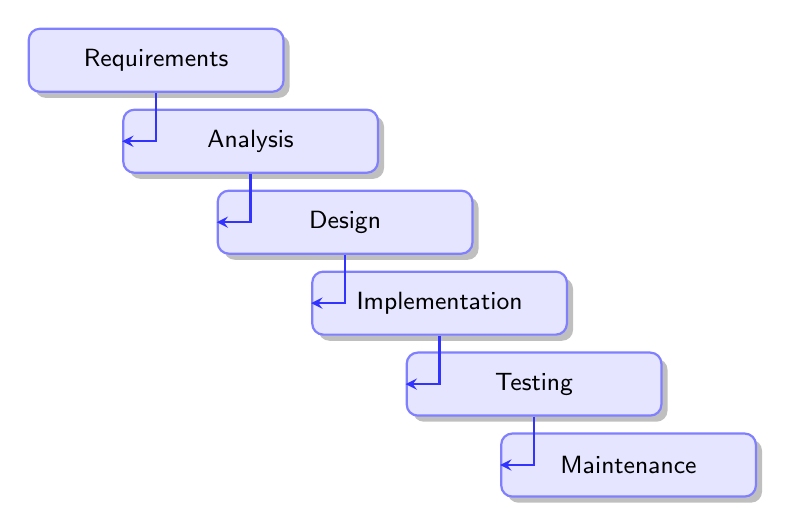
\begin{tikzpicture}[
        auto,
        every node/.style={
            rectangle, rounded corners, draw=blue!50, fill=blue!10, thick,
            text width=3cm, align=center, font=\small, drop shadow, minimum height=0.8cm
        },
        arrow/.style={->, >=stealth, thick, color=blue!80}
    ]
        % Cascading nodes
        \node (req) {Requirements};
        \node (ana) [below=0.2cm of req, xshift=1.2cm] {Analysis};
        \node (des) [below=0.2cm of ana, xshift=1.2cm] {Design};
        \node (imp) [below=0.2cm of des, xshift=1.2cm] {Implementation};
        \node (tst) [below=0.2cm of imp, xshift=1.2cm] {Testing};
        \node (mnt) [below=0.2cm of tst, xshift=1.2cm] {Maintenance};

        % Connectors
        \draw[arrow] (req.south) |- (ana.west);
        \draw[arrow] (ana.south) |- (des.west);
        \draw[arrow] (des.south) |- (imp.west);
        \draw[arrow] (imp.south) |- (tst.west);
        \draw[arrow] (tst.south) |- (mnt.west);

    \end{tikzpicture}
    
    \vspace{0.3cm}
    \scriptsize{Sequential flow: Output of one phase is the input for the next.}
\end{frame}

% V-Model diagram
\begin{frame}[fragile]
    \frametitle{The V-Model}
    \centering
    \resizebox{0.95\textwidth}{!}{% Resize to fit
    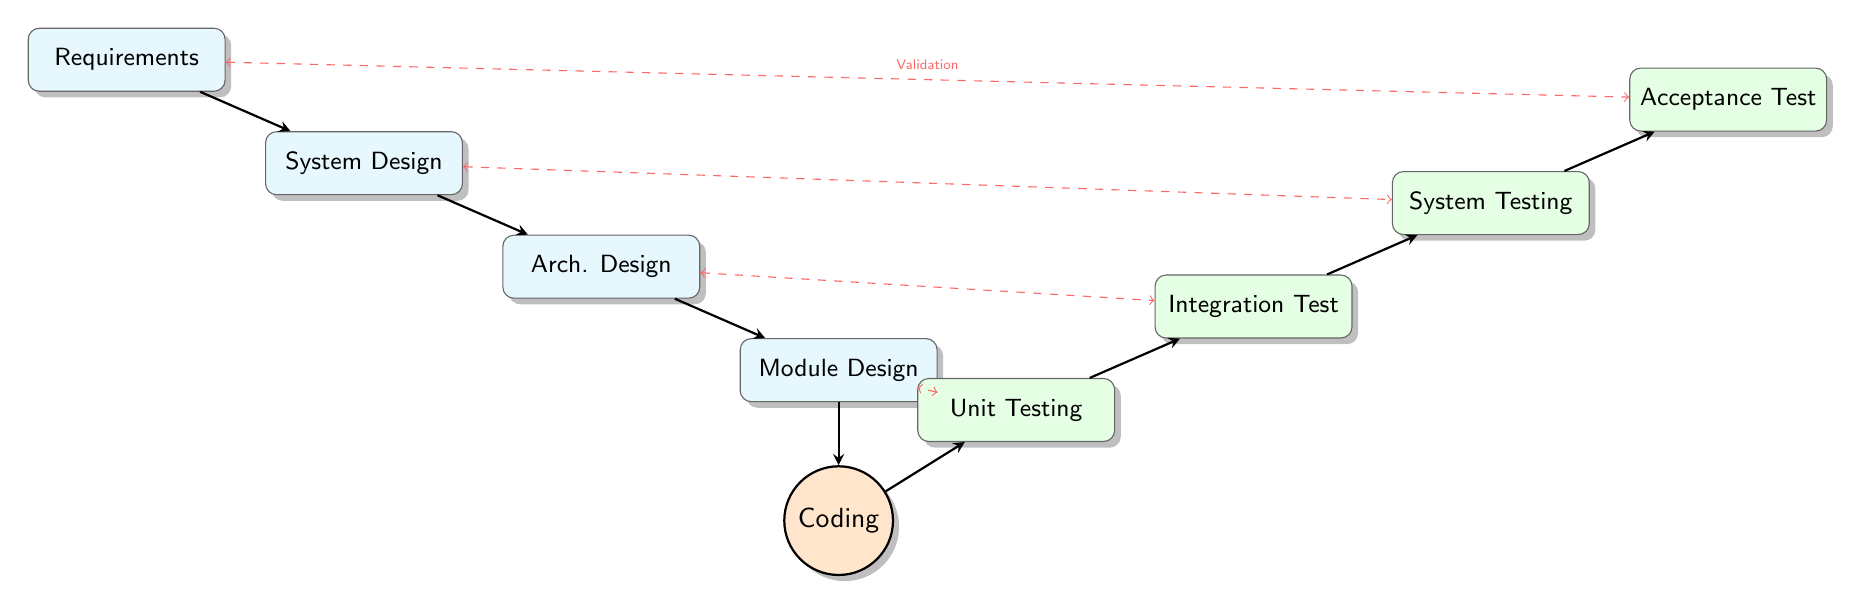
\begin{tikzpicture}[
        node distance=1.5cm,
        phase/.style={
            rectangle, draw=black!60, fill=cyan!10, rounded corners, 
            minimum width=2.5cm, minimum height=0.8cm, align=center, drop shadow, font=\small
        },
        val/.style={
            rectangle, draw=black!60, fill=green!10, rounded corners, 
            minimum width=2.5cm, minimum height=0.8cm, align=center, drop shadow, font=\small
        },
        arrow/.style={->, >=stealth, thick}
    ]
        % Left side
        \node[phase] (req) {Requirements};
        \node[phase, below right=0.5cm and 0.5cm of req] (sys) {System Design};
        \node[phase, below right=0.5cm and 0.5cm of sys] (arch) {Arch. Design};
        \node[phase, below right=0.5cm and 0.5cm of arch] (mod) {Module Design};
        
        % Bottom
        \node[circle, draw, fill=orange!20, thick, below=0.8cm of mod, drop shadow] (code) {Coding};
        
        % Right side
        \node[val, above right=0.5cm and 0.5cm of code] (unit) {Unit Testing};
        \node[val, above right=0.5cm and 0.5cm of unit] (int) {Integration Test};
        \node[val, above right=0.5cm and 0.5cm of int] (syst) {System Testing};
        \node[val, above right=0.5cm and 0.5cm of syst] (acc) {Acceptance Test};

        % Flow arrows
        \draw[arrow] (req) -- (sys);
        \draw[arrow] (sys) -- (arch);
        \draw[arrow] (arch) -- (mod);
        \draw[arrow] (mod) -- (code);
        
        \draw[arrow] (code) -- (unit);
        \draw[arrow] (unit) -- (int);
        \draw[arrow] (int) -- (syst);
        \draw[arrow] (syst) -- (acc);

        % Validation lines
        \draw[dashed, <->, red!60] (req) -- (acc) node[midway, above, font=\tiny] {Validation};
        \draw[dashed, <->, red!60] (sys) -- (syst);
        \draw[dashed, <->, red!60] (arch) -- (int);
        \draw[dashed, <->, red!60] (mod) -- (unit);

    \end{tikzpicture}
    }
\end{frame}

% Incremental
\begin{frame}[fragile]
    \frametitle{Incremental Model}
    \centering
    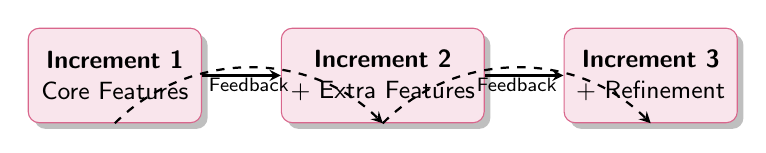
\begin{tikzpicture}[
        every node/.style={font=\small},
        inc/.style={rectangle, draw=purple!60, fill=purple!10, rounded corners, minimum width=2.2cm, minimum height=1.2cm, align=center, drop shadow},
        arrow/.style={->, >=stealth, thick}
    ]
        \node[inc] (i1) {\textbf{Increment 1} \\ Core Features};
        \node[inc, right=1cm of i1] (i2) {\textbf{Increment 2} \\ + Extra Features};
        \node[inc, right=1cm of i2] (i3) {\textbf{Increment 3} \\ + Refinement};
        
        % Arrows
        \draw[arrow] (i1) -- (i2);
        \draw[arrow] (i2) -- (i3);
        
        % Feedback loops
        \draw[arrow, dashed, bend left=45] (i1.south) to node[below, font=\scriptsize] {Feedback} (i2.south);
        \draw[arrow, dashed, bend left=45] (i2.south) to node[below, font=\scriptsize] {Feedback} (i3.south);

    \end{tikzpicture}
    
    \vspace{0.5cm}
    \raggedright
    \small System is broken down into small, manageable portions. Functional software is produced early.
\end{frame}

% Spiral
\begin{frame}[fragile]
    \frametitle{Spiral Model}
    \centering
    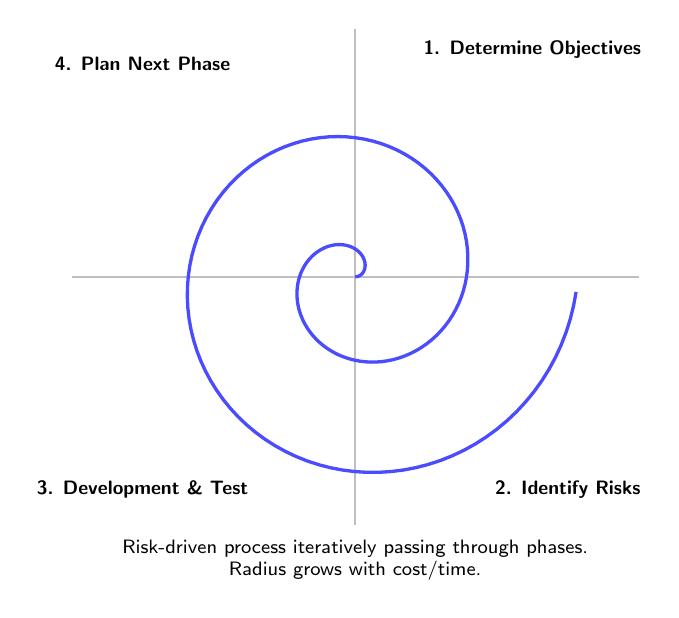
\begin{tikzpicture}[scale=0.9, font=\scriptsize, >=stealth]
        % Axes
        \draw [thick, gray!50] (-4,0) -- (4,0);
        \draw [thick, gray!50] (0,-3.5) -- (0,3.5);
        
        % Quadrant Labels
        \node at (2.5, 3.2) {\textbf{1. Determine Objectives}};
        \node at (3, -3) {\textbf{2. Identify Risks}};
        \node at (-3, -3) {\textbf{3. Development \& Test}};
        \node at (-3, 3) {\textbf{4. Plan Next Phase}};
        
        % Spiral
        \draw [blue!70, very thick, domain=0:12.5, samples=200] plot ({\x r}: {0.25*\x});
        
        % Annotation
        \node[align=center] at (0, -4) {Risk-driven process iteratively passing through phases.\\Radius grows with cost/time.};
    \end{tikzpicture}
\end{frame}

% Agile / Scrum
\begin{frame}[fragile]
    \frametitle{Agile (Scrum) Process}
    \centering
    \resizebox{\textwidth}{!}{
    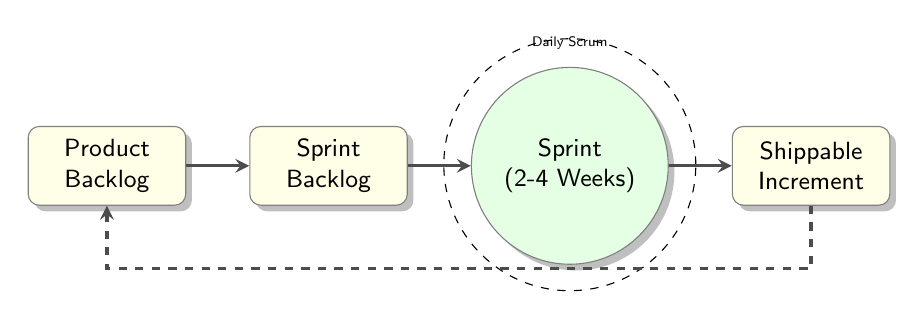
\begin{tikzpicture}[
        node distance=0.8cm,
        box/.style={rectangle, draw=black!50, fill=yellow!10, rounded corners, align=center, font=\small, drop shadow, minimum height=1cm, minimum width=2cm},
        circlebox/.style={circle, draw=black!50, fill=green!10, align=center, font=\small, drop shadow, minimum size=2.5cm},
        arrow/.style={->, >=stealth, very thick, color=black!70}
    ]
        \node[box] (backlog) {Product \\ Backlog};
        \node[box, right=of backlog] (sprintback) {Sprint \\ Backlog};
        
        \node[circlebox, right=of sprintback] (sprint) {Sprint \\ (2-4 Weeks)};
        \node[above=0.1cm of sprint, font=\tiny] {Daily Scrum};
        \node[circle, draw, dashed, minimum size=3.2cm, above=-2.85cm of sprint] (cycle) {};

        \node[box, right=of sprint] (shippable) {Shippable \\ Increment};

        % Arrows
        \draw[arrow] (backlog) -- (sprintback);
        \draw[arrow] (sprintback) -- (sprint);
        \draw[arrow] (sprint) -- (shippable);
        
        % Return arrow
        \draw[arrow, dashed] (shippable.south) -- +(0,-0.8) -| (backlog.south);
        
    \end{tikzpicture}
    }
    \vspace{0.5cm}
    \small Iterative development, constant feedback, flexible to change.
\end{frame}


\begin{frame}
    \frametitle{Next Steps}
    \begin{itemize}
        \item \textbf{This Week's Workshop:} Learning Git (Version Control).
        \item \textbf{Reading:} Sommerville, \textit{Software Engineering 9th Edition}, Chapter 1.
        \item \textbf{Next Week:} Software Process \& Project Planning.
    \end{itemize}
\end{frame}

\begin{frame}
    \frametitle{Q \& A}
    \begin{center}
        \Huge Any Questions?
    \end{center}
\end{frame}

\end{document}